\documentclass[preprint,nocopyrightspace]{sigplanconf}

\usepackage{graphicx,color}
\usepackage{subfigure}
\usepackage{amsmath}
\usepackage{amsfonts}
\usepackage{amssymb}
\usepackage{amsthm}
\usepackage{listings}
\usepackage{xspace}
\usepackage{paralist}
\usepackage{array}
\usepackage{booktabs}
\usepackage{balance}
\usepackage[vlined,ruled,linesnumbered]{algorithm2e}
\usepackage{algorithmic}

% Needed to rename {algorithm} wrapped {algorithmic} sections.
\usepackage{float}

% Used for theorem formatting.
\usepackage{amsthm}

% Graphs & figures.
\usepackage{tikz}
\usetikzlibrary{arrows,backgrounds,snakes}

\usepackage[sort&compress]{natbib}

% hyperref redefines a number of macros, so it should be last.  Empirically,
% doing so eliminates compiler warnings.
\usepackage[bookmarks, colorlinks]{hyperref}
% According to the hyperref readme, algorithm must follow hyperref

%~~~~~~~~~~~~~~~~~~~~~~~~~~~~~~~~~~~~~~~~~~~~~~~~~~~~~~~~~~~~~~~~~~~~~~~~~~~~~~
% Macros																{{{1

% English
\newcommand{\cf}{\hbox{\emph{cf.}}\xspace}
\newcommand{\deletia}{\ldots [deletia] \ldots}
\newcommand{\etal}{\hbox{\emph{et al.}}\xspace}
\newcommand{\eg}{\hbox{\emph{e.g.}}\xspace}
\newcommand{\ie}{\hbox{\emph{i.e.}}\xspace}
\newcommand{\scil}{\hbox{\emph{sc.}}\xspace} %scilicet: it is permitted to know
\newcommand{\st}{\hbox{\emph{s.t.}}\xspace}
\newcommand{\wrt}{\hbox{\emph{w.r.t.}}\xspace}
\newcommand{\etc}{\hbox{\emph{etc.}}\xspace}
\newcommand{\viz}{\hbox{\emph{viz.}}\xspace} %videlicet: it is permitted to see
\newcommand{\vs}{\hbox{\emph{vs.}}\xspace}

\newcommand{\Projn}{NAND\xspace}

\newcommand{\todo}[1]{{\color{red}#1}}
\newcommand{\kp}[1]{\todo{Karen: #1}}
\newcommand{\eb}[1]{\todo{Earl: #1}}

\newcommand{\ourtitle}{\Projn: Smashing Heisentests}

\newcommand{\avgoverhead}{$7\%$\xspace} %average overhead rate seen as a percentage
\newcommand{\avgdatarate}{$0.6$\,{\small MB/s}\xspace} %average data logging rate

\newcommand{\maxoverhead}{$11\%$\xspace} %largest overhead rate seen as a percentage
\newcommand{\maxdatarate}{$1.3$\,{\small MB/s}\xspace} %largest data logging rate

\newcommand{\avgoverheadbase}{$14\%$\xspace} %average BASELINE overhead rate seen as a percentage
\newcommand{\avgdataratebase}{$2.2$\,{\small MB/s}\xspace} %average BASELINE data logging rate

\newcommand{\maxoverheadbase}{$22\%$\xspace} %largest BASELINE overhead rate seen as a percentage
\newcommand{\maxdataratebase}{$5.6$\,{\small MB/s}\xspace} %largest BASELINE data logging rate

\newcommand{\averagereverse}{$0.29s$\xspace} %average reverse execution time
\newcommand{\maxreverse}{$0.68s$\xspace} %max reverse execution time

\newcommand\bench[1]{\textsf{\small #1}}

%% Document-specific hyperref options
\hypersetup{
pdftitle={\ourtitle},
    pdfauthor={Earl T. Barr and Morrison Cole},
    plainpages=false,
    linkcolor=blue, % Overriding these colors to black is somewhat unfortunate
    %citecolor=black, % b/c the defaults are useful in color.
    citecolor=blue, % b/c the defaults are useful in color.
    filecolor=black,
    urlcolor=blue,
    pdfpagelabels
}
\def\sectionautorefname{Section}
\def\subsectionautorefname{Section}
\def\subsubsectionautorefname{Section}
\newcommand{\subfigureautorefname}{\figureautorefname} %for subfigures
\newcommand{\defref}[1]{\hyperref[#1]{Definition~\ref*{#1}}}
\newcommand{\algref}[1]{\hyperref[#1]{Algorithm~\ref*{#1}}}
\newcommand{\lineref}[1]{\hyperref[#1]{Line~\ref*{#1}}}

%\setlength\textfloatsep{4mm}

%% lstlisting
\lstset{
	basicstyle=\ttfamily\small,
	numbers=left,
	language=Java,
	captionpos=b,
	breaklines=true,
	escapeinside={(*@}{@*)},
	breakatwhitespace=true
}

% show paper number for submission
\pagestyle{plain}
\pagenumbering{arabic}

\conferenceinfo{XXX}{YYY.}
\copyrightyear{ZZZZ}
\copyrightdata{WWWW}

\preprintfooter{Draft}
\titlebanner{DRAFT---Do not distribute}

\title{\ourtitle \vspace{-5mm}}

\authorinfo{Earl T. Barr \and Morrison Cole}
		{University College London}
    {\texttt{\{e.barr,morrison.cole.10\}@ucl.ac.uk}}

%\authorinfo{}
%		{}
%		{}

\begin{document}

\maketitle

\begin{abstract}

We present a framework for identifying and accelerating the resolution of flaky test cases in a test suite. A flaky test case is one whose outcome is sensitive to some unknown input.

The framework operates on a continuous lifecycle. To begin, each test's probability of failure is calculated. Then, each test is adaptively instrumented with respect to a budget --- state-logging probes are placed in choice locations. Finally, aggregated data is analysed to identify predicates strongly associated with test failure. At each stage, the framework can work autonomously or with input from a developer.

Our instrumentation approach applies bug isolation techniques in an ideal environment, allowing us to record and analyse a huge amount of runtime data over time. We improve probe placement by taking into account control flow graphs and loops. Finally, we introduce the notion of an instrumentation budget and allocate probes based on learned cost.

We discuss and document the implementation of a working proof of concept, named \textit{\splatter}, that targets Android applications and integrates with a popular open-source continuous integration tool. We present preliminary results from the use of the tool on tests from a commercial product's test suite.

\end{abstract}


%\category{D.3.3}{Programming Languages}
%{Language Constructs and Features}
%\terms Some Terms Here
%\keywords Some Keywords Here

\vspace*{4mm}
\noindent``\todo{find appropriate quote.} Debugging involves backwards reasoning''

\hfill Brian Kernighan and Rob Pike

\hfill The Practice of Programming, 1999

\section{Introduction}
\label{sec:intro}

\textit{The following are placeholders; subsections are to be removed.}

\subsection{Testing is used in practice across the industry}

Testing is as much a part of modern software development as deployment. Enforces quality, prevents regressions, reduces need for manual testing in certain areas.

\subsection{Testing is flawed/not always reliable}

Flaky tests across the industry.

\subsection{What we intend to do}

Apply adaptive bug isolation techniques to testing to gather information on flaky test cases with the aim of aiding their stabilization.

\subsection{How the rest of the paper is structured}
\section{Example}
\label{sec:example}

TODO: Example from Shazam's codebase.

\section{Approach}
\label{sec:approach}


\subsection{Fixing flaky tests}

\todo{Have a comparison between the results gathered normally (logs + assertion failure/stacktrace + screenshot) and heisentest (JSON logs).There are strong ties to ‘heisenbugs’ and ‘debuggability’ here. Perhaps get references.}

Sometimes, it is not possible to fix a flaky test from the information output by the testrunner alone. Typically, the information includes logs, an assertion failure message and/or a stack trace. Applications with a user interface may also provide a number of screenshots. Often, a developer will have to manually gather information to build up an understanding of the intended flow vs. the actual flow on failing runs. For flaky tests with a low failure rate, this can be a painstaking and time-consuming process. Indeed, if the flaky test is a timing based issue, attaching a debugger may cause the test to pass indefinitely.

\todo{Have a comparison between the results gathered normally (logs + assertion failure/stacktrace + screenshot) and heisentest (JSON logs).}


\subsection{Aims and Goals}

Flaky tests are hard to fix. In general, there are three stages during which we may intervene:
\begin{enumerate}
	\item Identification - which tests in the suite are flaky?
	\item Prioritisation - why of the flaky tests should we fix first?
	\item Resolution - what information can we gather to speed the resolution of a test?
\end{enumerate}

Ultimately, the final stage is the target. In order to tackle the problem practically, knowledge gathered at each stage must be combined and considered.

Existing tools (Shazam’s Flaky Test Monitor included) provide answers to 1. This information can be used to inform manual inspection of 2. As of yet, no tool exists to tackle 3.

In a typical software development project, continuous integration systems will be set up from the beginning. Developers write code and commit to source control. A master server will detect the change and assign one of a number of build agents (other servers with the capability to build the project(s) - virtual or otherwise) an attached job.

For a typical job, the chosen build agent pulls down the latest changes, compiles and run the tests and runs any post-build tasks. At the end, any build artifacts (distributable packages, test results, etc.) will be uploaded to the master server and the agent will be once again free to build the next iteration. Note that in reality, a job can comprise of any number of runnable steps - from executing a shell script to hitting an external server.

\todo{A diagram of this flow would be nice.}

It is obvious that, if we are to develop a tool to assist developers with flaky tests, we should run as part of a modular continuous integration system.


\subsection{Formal Definition of a Flaky Test}

\theoremstyle{definition}
\newtheorem{defn}{Definition}[section]

% Noticed that 'A Hueristic Test Data Generation Approach for Program Fault Localization' has a nice definition for passing/failing test cases (no notion of flakiness though). See section 3.1, Definition 1.

\begin{defn}
	Given a subject under test $f: \vec{I} -> \vec{O}$.

	A test case is $(\vec{i},\vec{o})$

	The “fixed f” condition needs fixing.  It will need to be wrt the slice from the program point at which $\vec{o}$ is generated to entry, given $\vec{i}$. In others words, it’s impact analysis.  Intuitively, a test can only be flaky when its behavior is sensitive unknown inputs and not to changes to f that it, in fact, is designed to test.

	A \emph{flaky test case} is a test case where, for fixed $f$,
	$p(f(\vec{i} = \vec(o)) = 1 - \epsilon$

	Remark: A flaky test case is an unfair coin.

	Let $\vec{I}$ be the lifting of all inputs, including coin flips and environmental interactions, into a single input vector.

	The key is the true $\vec{I}$ is only partially known;  we capture flakiness as unknown components of $\vec{I}$, like Todd Mytkowicz’ sensitivity to the length of environmental variables, etc.

	Note:  formalize how much data we will need to gather in order to discover the cause of flakiness as a function of epsilon.  Rare events, like flakiness, are related to smoothing.

	Combined with our budget b, we can determine what values of $\epsilon$ we can afford to detect!
\end{defn}

% See: http://www.texample.net/tikz/examples/line-plot-example/
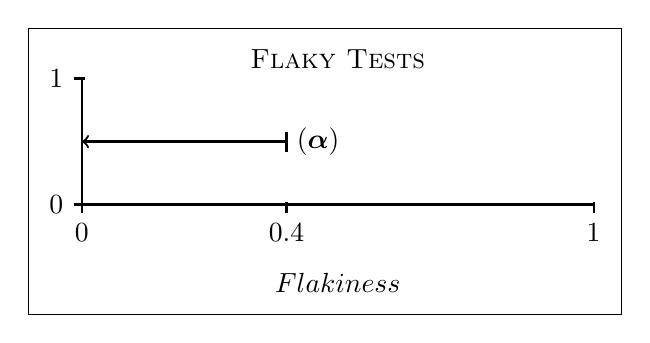
\begin{tikzpicture}[thick, framed, x=6.5cm, y=1.6cm]
	% Title
	\draw (0.5, 1) node[above] {$\textsc{Flaky Tests}$};

	% Axis
	\draw (0,0) -- coordinate (x axis mid) (1,0);
    \draw (0,0) -- coordinate (y axis mid) (0,1);

    % Axis Labels
    \node (padding) [below] at (0.4, 0) {};
	\node[below of = padding] at (x axis mid) {$Flakiness$};

    % Ticks
    \foreach \x in {0, 0.4, 1}
    	\draw (\x, 1pt) -- (\x, -3pt) node[anchor=north] {\x};
    \foreach \y in {0, 1}
    	\draw (1pt, \y) -- (-3pt, \y) node[anchor=east] {\y};

	% Flaky test range
    \draw[<-] (0, 0.5) -- (0.4, 0.5); % Draw horizontal line
    \draw (0.4, 0.42) -- (0.4, 0.58); % Draw right vertical tab

    % Alpha label
    \node [right] at (0.4, 0.5) {$(\boldsymbol{\alpha})$};
\end{tikzpicture}


Test suite $f$ with flaky tests $f!$.
Budget $B_{f} = B_{6} + B_{f!} + B_{nd}$

\paragraph{Instrumentation pseudocode:}

% Use 'in' for-loop range notation rather than 'to'.
\renewcommand{\algorithmicto}{\textbf{in}}

% The {algorithm} wrapper is pretty unattractive as far as I'm concerned.
% Need to look into alternative ways of formatting this.
\begin{algorithm}
\caption{Allocate instrumentation budget across a test suite}
\label{alg1}
\begin{algorithmic}
	% Perhaps this should just take a single tests[]. We can query the element to determine its 'priority' (relative flakiness).
	% Or, could take a vector<test, flakiness> to be explicit.
	\STATE{\textbf{splatter} (budget, flakyTests[], allTests[])}
	\STATE{}
	\COMMENT{Need a function that looks at all the tests and their associated priorities, orders them and attaches an allowedBudget value in terms of the whole budget}
 	\WHILE{$budget \geq 0$}
 		% Simpler if the 'instrumentTest' function returns a value representing the amount of budget it actually used, rather than its remainder.
 		\STATE{$budget \gets budget - allowedBudget + \textbf{instrumentTest} (test, allowedBudget)$}
	\ENDWHILE
\end{algorithmic}
\end{algorithm}

\begin{algorithm}
\caption{Instrument a test with respect to a given budget}
\label{alg2}
\begin{algorithmic}
	\STATE{\textbf{instrumentTest} (test, budget)}
	% Should 'sites' just be a parameter?
	\STATE{$sites \gets test.instrumentationSites$}
	\FOR{$site$ \TO $sites$}
		% Should probably define a cost function (e.g. cost(instrumentationPoint)) and use that, rather than using an unexplained accessor.
		\STATE{$cost \gets site.cost$}
		\IF{$cost \le budget$}
			\STATE{$site.active \gets true$}
			\STATE{$budget \gets budget - cost$}
		\ELSE
			% Need to work out how to define new algorithmic-style macros (e.g. \BREAK)
			\STATE{\textbf{break}}
		\ENDIF
	\ENDFOR
	\RETURN{budget}
\end{algorithmic}
\end{algorithm}

% Focus on the interesting design decisions. For example, what were the alternatives, why select one particular solution?
% Don't flood the chapter with diagrams. Be selective.
% Avoid lengthy sections of code; use pseudo-code.
% This is a core chapter and will usually be quite substantial, 10 pages or more.
\section{Design and Implementation}
\label{sec:imp}

\begin{framed}
	\begin{itemize}
		\item Describe the design of what you have created.
		\item Start with the application architecture, giving its overall structure and the components that make up that structure.
		\item Give a description of the design of each of the components that make up the architecture.
		\item Include the database or storage representation.
		\item Provide implementation details as necessary.
	\end{itemize}
\end{framed}

\section{Evaluation}
\label{sec:eval}

\subsection{The problem is real: it occurs in real world test suites. The goal is to quantify the problem for the skeptical reviewer.}

\subsection{How serious/extensive is the problem?}

\subsection{We solve the problem}

\section{Related Work}
\label{sec:relwork}

Liblit’s Adaptive Bug Isolation [] and other papers have taken a conservative
approach to information gathering. The projects have targeted production code,
so privacy and performance are major concerns.

\todo{Citations - there are a lot to add here!}

\subsubsection{Ordering}

In previous statistical bug isolation projects, ordering is completely discarded
due to privacy concerns []. Recording a play-by-play execution is invasive to
the common user.

Since our instrumentation will run in a development environment, there are no
user concerns - the tests are automated. We can maintain ordering with a little
more overhead.

Multi-threaded environments are commonplace. In order to record the execution
order of multiple threads, we include the system time in each log event. Each
thread logs to a separate sink. After the tests run completes, we merge and
interleave the individual logs before storing them. We end up with a single log
file with times and thread IDs.

\subsubsection{Storage/Result Collection}

Again, the context of our execution allows more flexibility. In production
systems, logs have to be stored on user devices and (eventually) transferred to
a central location for analysis. User storage space and bandwidth is precious,
so it is essential to minimise both.

In our case, tests will be run internally on project-owned machines and devices.
Log files can be transferred to the central database immediately following a
test run. Each test run by definition requires a clean device, so build agents
will almost certainly never run out of space since they will at any moment be
storing the logs from at most one test run.

The only real storage concern is that of the central database. But, this can be
managed effectively by limiting the number of historical test run logs to keep -
much in the same way Jenkins and other CI tools do by default.

\subsubsection{Performance}

Instrumentation adds performance overhead. In the case of a production system,
this is a major problem since performance directly affects a user’s experience.
Nainar and Liblit \cite{ArumugaNainar:2010:ABI:1806799.1806839} propose an
adaptive bug isolation system with a performance overhead of just 1\%.

In a test environment, smoothness and load times rarely matter. Of course, there
are exceptions (performance regression tests, etc.), but we expect to mainly be
dealing with system tests. We can safely add instrumentation and ignore
performance, unless it begins to affect the thread-wise execution. If a \flaky
test begins consistently passing when heavily instrumented, we can simply reduce
the instrumentation until the previous \flaky behaviour is once again observed.

\subsubsection{Adaptivity}

Both fixed and adaptive approaches have been proposed[] in the past. All of
these approaches were developed with the underlying constraint of deploying the
instrumented software to real users. [adaptive bug isolation] makes use of
binary instrumentation to iteratively re-instrument deployed applications to
hone in on a bug-predicting predicates. Whilst the adaptive approach has many
benefits in terms of overhead, it relies on a specialized API - Dyninst - for
code patching to support the injection of  instrumentation at runtime. This has
additional runtime costs \cite{DyninstGuide} associated with saving and
restoring registers and performing protective checks not present in a fixed
instrumentation.

Again, our context allows more freedom. Every run requires a new build by
nature, so simply apply a unique fixed instrumentation every time. In other
words, we retain the optimisation benefits of a fixed instrumentation whilst
gaining those of the adaptive solution.

% This chapter is typically 204 pages long but could be longer if the project work requires more extensive evaluation.
\section{Conclusion}
\label{sec:conc}

\begin{itemize}
	\item A summary of what the project has achieved. Address each goal set out in the introduction.
	\item A critical evaluation of the results of the project (e.g., how well were the goals met, is the application fit for purpose, has good design and implementation practice been followed, was the right implementation technology chosen and so on).
	\item Future work. How could the project be developed if you had another 6 months.
	\item Wrap-up and final thoughts on your project.
\end{itemize}

%\listoftodos

\balance

\nocite{*}
\bibliographystyle{abbrv}
\bibliography{Bib/paper}

\end{document}
